\documentclass[11pt]{article}

\usepackage[T1]{fontenc}
\usepackage{lmodern}
\usepackage{microtype}
\usepackage{amsmath,amssymb,amsthm}
\usepackage{booktabs,tabularx,array,float,xcolor}
\usepackage{graphicx,longtable}
\usepackage{tikz}
\usetikzlibrary{calc}
\usepackage{titlesec}
\usepackage[a4paper,margin=27mm]{geometry}
\usepackage[colorlinks=true,linkcolor=blue!55!black,
  citecolor=blue!55!black,urlcolor=blue!55!black]{hyperref}

\newtheorem{theorem}{Theorem}
\newtheorem{proposition}[theorem]{Proposition}
\newtheorem{corollary}[theorem]{Corollary}
\newtheorem{conjecture}[theorem]{Conjecture}
\newtheorem{remark}[theorem]{Remark}
\newcommand{\ETC}{\mathrm{ETC}}
\newcommand{\Cev}{\mathcal T_1}
\newcommand{\Circ}{\mathcal T_2}
\newcommand{\Ped}{\mathcal T_3}
\titlespacing*{\section}{0pt}{2.5ex plus .7ex minus .2ex}{1.1ex}

\title{Triangle Centers Relative to Their Cevian, Circumcevian,\\
and Pedal Triangles}
\author{Ismail Hammoudeh}
\date{September 2026}

\begin{document}
\maketitle

\begin{abstract}
For a triangle center $P=X_i(ABC)$, we ask whether the same Euclidean point is
classified as $X_j$ relative to the cevian, circumcevian, or pedal triangle
of $P$.  Circumcevian--pedal similarity and its isogonal transfer principle
are classical; we give a self-contained coordinate proof and use them as the
organizing mechanism.  The algebraic contribution is an explicit branch
refinement for the classical family $F_\lambda$: under the positive-area
convention, the target parameter is $-\lambda$ when the source is inside
the circumcircle and $\lambda$ when it is outside.  This gives a general
near-equilateral obstruction to unrestricted fixed-point claims.  Affine
covariance of symmetric polynomials proves the fixed relations for
$X_{67371}$ and $X_{9181}$.  Classical relations involving the
Steiner-inellipse foci and $X_{187}$ are recovered by intrinsic proofs.

Using a local snapshot of the \emph{Encyclopedia of Triangle Centers} (ETC)
contiguous through $X_{72807}$, we enumerate every diagonal index and the two
directed off-diagonal strips $\min(i,j)\leq1000$.  The census distinguishes
exact identities, branch-dependent relations, numerical candidates, and
unavailable evaluations.  An audit corrects an acute-seed cache fallback,
and additional high-precision tests approach special shapes systematically.
The accompanying supplement contains the fixed data snapshot, readable
formulas, source programs, ordered test triangles, residuals, and a final
status table.
\end{abstract}

\noindent\textbf{Keywords.} triangle center; cevian triangle; circumcevian
triangle; pedal triangle; experimental geometry; Encyclopedia of Triangle
Centers.

\section{The geometric question}

Let $ABC$ be a labelled, nondegenerate scalene triangle and let $P$ be a
finite point distinct from the vertices.  Denote by
\begin{itemize}
\item $\Cev(P)=A_1B_1C_1$ the cevian triangle, with
  $A_1=AP\cap BC$ and cyclically;
\item $\Circ(P)=A_2B_2C_2$ the circumcevian triangle, where $A_2$ is the
  second intersection of $AP$ with the circumcircle and cyclically;
\item $\Ped(P)=A_3B_3C_3$ the pedal triangle, whose vertices are the
  perpendicular projections of $P$ on $BC,CA,AB$.
\end{itemize}
Only noncollinear derived triples are admitted.  We write
\begin{equation}\label{eq:coincidence}
 \mathcal C_k(i,j;ABC):\qquad
 X_i(ABC)=X_j\bigl(\mathcal T_k(X_i(ABC))\bigr).
\end{equation}
Thus $M_k:X_i\mapsto X_j$ records a reclassification of the \emph{same
Euclidean point in the ambient plane}; it is not an ordinary point map.
The case $i=j$ is called a fixed-point candidate.

An instance of \eqref{eq:coincidence} is \emph{admissible} if the source
defines a finite real point, the required traces are finite, the derived
vertices are distinct and noncollinear, and the target defines a finite
real point on its specified ETC branch.  A zero homogeneous triple is
undefined; it is not a point at infinity.  Common rational factors are
cancelled before interpreting a formula, but no continuation of a selected
algebraic root is imposed unless stated.  An unrestricted identity means
equality at every admissible instance of its stated real domain, not
existence on every triangle.

Figure~\ref{fig:three-constructions} summarizes the three changes of
reference triangle.  It is schematic rather than metrically exact.

\begin{figure}[ht]
\centering
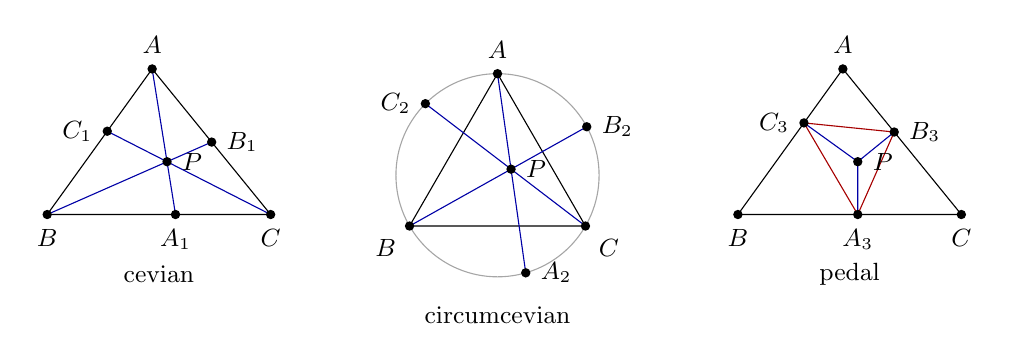
\begin{tikzpicture}[scale=.86,every node/.style={font=\small},
  point/.style={circle,fill=black,inner sep=1.2pt}]
\begin{scope}[xshift=0cm]
  \coordinate (A) at (0,2.15); \coordinate (B) at (-1.55,0);
  \coordinate (C) at (1.75,0); \coordinate (P) at (.22,.78);
  \coordinate (A1) at (.345,0); \coordinate (B1) at (.879,1.070);
  \coordinate (C1) at (-.663,1.230);
  \draw (A)--(B)--(C)--cycle;
  \draw[blue!65!black] (A)--(A1) (B)--(B1) (C)--(C1);
  \node[point,label=right:$P$] at (P) {};
  \foreach \Q/\pos/\lab in {A/above/$A$,B/below/$B$,C/below/$C$,
    A1/below/$A_1$,B1/right/$B_1$,C1/left/$C_1$}
    \node[point,label=\pos:\lab] at (\Q) {};
  \node at (.1,-.88) {cevian};
\end{scope}
\begin{scope}[xshift=5.1cm]
  \coordinate (O) at (0,.58); \coordinate (A) at (0,2.08);
  \coordinate (B) at (-1.299,-.17); \coordinate (C) at (1.299,-.17);
  \coordinate (P) at (.20,.67);
  \draw[gray!70] (O) circle (1.5);
  \draw (A)--(B)--(C)--cycle;
  \draw[blue!65!black] (A)--(.417,-.861) (B)--(1.318,1.296)
    (C)--(-1.065,1.637);
  \node[point,label=right:$P$] at (P) {};
  \node[point,label=above:$A$] at (A) {};
  \node[point,label=below left:$B$] at (B) {};
  \node[point,label=below right:$C$] at (C) {};
  \node[point,label=right:$A_2$] at (.417,-.861) {};
  \node[point,label=right:$B_2$] at (1.318,1.296) {};
  \node[point,label=left:$C_2$] at (-1.065,1.637) {};
  \node at (0,-1.48) {circumcevian};
\end{scope}
\begin{scope}[xshift=10.2cm]
  \coordinate (A) at (0,2.15); \coordinate (B) at (-1.55,0);
  \coordinate (C) at (1.75,0); \coordinate (P) at (.22,.78);
  \coordinate (A3) at ($(B)!(P)!(C)$);
  \coordinate (B3) at ($(C)!(P)!(A)$);
  \coordinate (C3) at ($(A)!(P)!(B)$);
  \draw (A)--(B)--(C)--cycle;
  \draw[blue!65!black] (P)--(A3) (P)--(B3) (P)--(C3);
  \draw[red!65!black] (A3)--(B3)--(C3)--cycle;
  \node[point,label=right:$P$] at (P) {};
  \foreach \Q/\pos/\lab in {A/above/$A$,B/below/$B$,C/below/$C$,
    A3/below/$A_3$,B3/right/$B_3$,C3/left/$C_3$}
    \node[point,label=\pos:\lab] at (\Q) {};
  \node at (.1,-.88) {pedal};
\end{scope}
\end{tikzpicture}
\caption{The three derived reference triangles in
\eqref{eq:coincidence}.}
\label{fig:three-constructions}
\end{figure}

If $P$ is on the circumcircle, $\Circ(P)$ collapses to $P,P,P$, while
$\Ped(P)$ is collinear by the Simson theorem.  Neither configuration admits
an ETC target center.  Selected-root definitions may also change branch as
the triangle shape or its labelling changes.  These facts motivate the
degeneracy checks and multiple-shape audits below.

\section{Classical transfer principle and exact construction}

Let $P=(u:v:w)$ in barycentric coordinates of $ABC$, with side lengths
$a=BC$, $b=CA$, $c=AB$.  The cevian traces are
\[
 A_1=(0:v:w),\qquad B_1=(u:0:w),\qquad C_1=(u:v:0).
\]
The circumcircle has barycentric equation
\[
 a^2yz+b^2zx+c^2xy=0.
\]
Intersecting this equation with $AP$ and removing the known root $A$ gives
\begin{equation}\label{eq:circumcevian}
 A_2=\bigl(a^2vw:-v(b^2w+c^2v):-w(b^2w+c^2v)\bigr),
\end{equation}
with $B_2,C_2$ obtained cyclically.  The implementation constructs all three
derived triangles independently in Cartesian coordinates; equation
\eqref{eq:circumcevian} is an exact audit of the line-circle calculation.

The circumcevian and pedal problems are not independent.  The following
theorem provides the algebraic bridge between them.

\begin{theorem}[Circumcevian--pedal isogonal transfer]
\label{thm:isogonal-transfer}
Let $P=(u:v:w)$ be admissible, with $uvw(u+v+w)\ne0$, and suppose that
$\Circ(P)$ and $\Ped(P)$ are nondegenerate.  Under the correspondence
$A_2\leftrightarrow A_3$, $B_2\leftrightarrow B_3$,
$C_2\leftrightarrow C_3$, the two derived triangles have proportional
corresponding squared side lengths.  Moreover, the barycentric coordinate
triples of the same point $P$ in these triangles are isogonal conjugates.
Consequently, for every side-defined center function $X_j$ on a consistent
branch,
\begin{equation}\label{eq:isogonal-transfer}
 P=X_j(\Circ(P))
 \quad\Longleftrightarrow\quad
 P=\iota(X_j)(\Ped(P)).
\end{equation}
\end{theorem}

\begin{proof}
Put $A=a^2$, $B=b^2$, $C=c^2$ and $t=u+v+w$.  Let $R_A,R_B,R_C$ denote
the three raw triples supplied by \eqref{eq:circumcevian}, and let
$s_A,s_B,s_C$ be their coordinate sums.  Direct multiplication gives
\[
 uR_A+vR_B+wR_C
 =-(Avw+Bwu+Cuv)(u,v,w).
\]
Since $A_2=R_A/s_A$ and cyclically, the coordinates of $P$ relative to its
circumcevian triangle are therefore
\begin{equation}\label{eq:P-in-circ}
 P_{\Circ}=(us_A:vs_B:ws_C).
\end{equation}
The barycentric distance formula also gives
\[
 PA^2=-\frac{s_A}{t^2},\qquad
 PB^2=-\frac{s_B}{t^2},\qquad
 PC^2=-\frac{s_C}{t^2}.
\]
Thus \eqref{eq:P-in-circ} may be written
\begin{equation}\label{eq:P-in-circ-distance}
 P_{\Circ}=(uPA^2:vPB^2:wPC^2).
\end{equation}

For comparison, the foot on $BC$ is
\[
 A_3=\frac{1}{2At}
 \bigl(0,\ u(A+B-C)+2Av,\ u(A+C-B)+2Aw\bigr),
\]
with the other feet obtained cyclically.  Inverting this affine matrix gives
the particularly simple triple
\begin{equation}\label{eq:P-in-pedal}
 P_{\Ped}=\left(\frac A u:\frac B v:\frac C w\right).
\end{equation}

Let $a_2=B_2C_2$, $a_3=B_3C_3$, let $\mathcal R$ be the circumradius of
$ABC$, and let $\Pi_P$ be the signed power of $P$ with respect to its
circumcircle.  The projection formula and the power-of-a-point theorem give
\[
 a_3^2=\frac{a^2PA^2}{4\mathcal R^2},
 \qquad
 a_2^2=\frac{\Pi_P^2a^2}{PB^2PC^2}.
\]
Hence
\[
 \frac{a_2^2}{a_3^2}
 =\frac{4\mathcal R^2\Pi_P^2}{PA^2PB^2PC^2},
\]
and the same factor occurs cyclically.  The corresponding side triples are
therefore proportional.  Isogonal conjugation of
\eqref{eq:P-in-circ-distance} inside $A_2B_2C_2$ yields
\[
 \left(\frac{a_2^2}{uPA^2}:
       \frac{b_2^2}{vPB^2}:
       \frac{c_2^2}{wPC^2}\right)
 \sim\left(\frac A u:\frac B v:\frac C w\right),
\]
which is exactly \eqref{eq:P-in-pedal}.  This proves the assertion.
\end{proof}

\section{Relation to previous circumcevian theory}
\label{sec:previous-theory}

The similarity of the circumcevian and pedal triangles under the natural
vertex correspondence is classical; it appears in Kimberling's treatment of
central triangles \cite{Kimberling1998}.  Stothers gave the corresponding
coordinate transfer theorem and tables of circumcevian classes
\cite{StothersPedal,StothersCircum}.  In particular, those tables already
contain the reciprocal centroid--Steiner-focus class, the invariant centers
$X_3,X_6,X_{187}$, the class $X_{36}\leftrightarrow X_{186}$, and the
one-parameter extraversion class
\[
 \{Q(\phi),Q(-\phi)\},\qquad
 Q(\phi)=(\sin A\sin(A+\phi):\sin B\sin(B+\phi):
 \sin C\sin(C+\phi)).
\]
Up to a projective scalar this is the present $F_\lambda$ family with
$\lambda=-\cot\phi$.  Gibert's related tables also organize centers with
trilinears of the form $\tan(A+t)$ and associated Brocard-axis families
\cite{GibertTable38}.

Accordingly, Theorem~\ref{thm:isogonal-transfer}, the Steiner-focus result,
and the $X_{187}$ relations below are included as self-contained recoveries
and as checks on notation.  The contribution developed here is more
specific: it distinguishes the signed, oriented identity from the usual
positive-Heron convention, gives an exact formula for the branch change,
uses it to disprove apparent global fixed points, proves the high-index fixed
point $X_{67371}$, and audits a modern ETC snapshot far beyond the classical
tables.

\section{\texorpdfstring{The exact $F_\lambda$ family and its branch locus}
{The exact F-lambda family and its branch locus}}
\label{sec:families}

\subsection{The oriented parameter-reversal law}

Put
\[
 H=\sqrt{(a+b-c)(a-b+c)(-a+b+c)(a+b+c)}=4[ABC]
\]
and
\[
 D_a=a^2-b^2-c^2,\qquad D_b=b^2-c^2-a^2,\qquad
 D_c=c^2-a^2-b^2.
\]
Define
\begin{equation}\label{eq:F-lambda}
 F_\lambda=
 \bigl(a^2(D_a+\lambda H):b^2(D_b+\lambda H):
 c^2(D_c+\lambda H)\bigr).
\end{equation}
Its trilinears are
\[
 (-\cos A+\lambda\sin A:-\cos B+\lambda\sin B:
 -\cos C+\lambda\sin C).
\]
In the oriented calculations choose a counterclockwise realization of
$ABC$, so $H=2\det(B-A,C-A)>0$.  For a derived labelled triangle $T=UVW$,
write $H_T^{\mathrm{or}}=2\det(V-U,W-U)$, and use a superscript ``or''
when this signed radical replaces the positive Heron radical.
For an arbitrary realization, multiply the derived determinant by
$\operatorname{sgn}\det(B-A,C-A)$ instead.  Thus orientation is relative
to the source; the positive-Heron statements below are independent of
the realization.

\begin{theorem}[Circumcevian parameter reversal]
\label{thm:F-reversal}
On the generic nondegenerate domain,
\begin{equation}\label{eq:F-circ-law}
 F_\lambda(ABC)=F_{-\lambda}^{\mathrm{or}}
 \bigl(\Circ(F_\lambda(ABC))\bigr).
\end{equation}
The identity extends after cancellation wherever both sides remain defined.
The exceptional loci include $3\lambda^2=1$ and the vanishing factors
displayed in the proof.
\end{theorem}

\begin{proof}
Set $A=a^2$, $B=b^2$, $C=c^2$, $S=A+B+C$; then
\[
 H^2=2AB+2BC+2CA-A^2-B^2-C^2,\qquad D_a=2A-S.
\]
Define cyclically
\begin{equation}\label{eq:q-family}
 q_a=(3\lambda^2-1)A-2\lambda^2S+2\lambda H,\qquad
 Q=(3\lambda^2+1)H-2\lambda S.
\end{equation}
Substitution of $u=A(D_a+\lambda H)$ and its cyclic companions into
\eqref{eq:circumcevian} shows that the coordinate sums of the raw
circumcevian triples are
\[
 s_A=BCH^2q_a,\qquad s_B=CAH^2q_b,\qquad s_C=ABH^2q_c.
\]
By \eqref{eq:P-in-circ}, the original point relative to its circumcevian
triangle therefore has coordinates
\begin{equation}\label{eq:F-relative-coordinates}
 \bigl((D_a+\lambda H)q_a:
       (D_b+\lambda H)q_b:
       (D_c+\lambda H)q_c\bigr).
\end{equation}

Let $A'=a_2^2$, $B'=b_2^2$, $C'=c_2^2$.  Exact reduction of the
barycentric distance formula gives
\begin{equation}\label{eq:derived-sides-q}
 A'=\delta q_a,\qquad B'=\delta q_b,\qquad C'=\delta q_c,\qquad
 \delta=\frac{ABCQ^2}{H^2q_aq_bq_c}.
\end{equation}
The determinant of the normalized circumcevian triples gives
\begin{equation}\label{eq:derived-oriented-H}
 H_2^{\mathrm{or}}=-\delta Q.
\end{equation}
Equivalently, its square follows from the factorization
\[
 2(q_aq_b+q_bq_c+q_cq_a)-q_a^2-q_b^2-q_c^2=Q^2.
\]
Finally,
\begin{equation}\label{eq:key-family-factor}
 q_a-q_b-q_c+\lambda Q
 =(3\lambda^2-1)(D_a+\lambda H),
\end{equation}
cyclically.  The first coordinate of $F_{-\lambda}^{\mathrm{or}}$ in the
derived triangle is, by \eqref{eq:derived-sides-q}--
\eqref{eq:derived-oriented-H},
\[
 A'(A'-B'-C'-\lambda H_2^{\mathrm{or}})
 =\delta^2q_a(q_a-q_b-q_c+\lambda Q).
\]
Equation \eqref{eq:key-family-factor} makes this proportional to the first
coordinate in \eqref{eq:F-relative-coordinates}; the other two coordinates
follow cyclically.
\end{proof}

The theorem contains, on the corresponding oriented ETC branches,
\[
 X_3=F_0,\quad X_{61}=F_{-\sqrt3},\quad X_{62}=F_{\sqrt3},\quad
 X_{371}=F_{-1},\quad X_{372}=F_1,
\]
and the limiting member $F_\infty=X_6$.  It therefore explains the
circumcevian rows $X_3\mapsto X_3$, $X_6\mapsto X_6$,
$X_{61}\mapsto X_{62}$, and $X_{371}\mapsto X_{372}$.

Let $\iota$ denote isogonal conjugation and put
\begin{equation}\label{eq:G-lambda}
 G_\lambda=\iota(F_\lambda)
 =\left(\frac1{D_a+\lambda H}:\frac1{D_b+\lambda H}:
 \frac1{D_c+\lambda H}\right).
\end{equation}

\begin{corollary}[Pedal parameter law]\label{cor:pedal-family}
On the same generic oriented domain,
\begin{equation}\label{eq:F-pedal-law}
 F_{-\lambda}(ABC)=G_\lambda^{\mathrm{or}}
 \bigl(\Ped(F_{-\lambda}(ABC))\bigr).
\end{equation}
\end{corollary}
\begin{proof}
Apply Theorem~\ref{thm:F-reversal} to $P=F_{-\lambda}$ and then apply
Theorem~\ref{thm:isogonal-transfer}.  For the signed convention, let
$\Pi_P$ be the source power and $\mathcal R$ the circumradius.
Determinants of the normalized derived vertex matrices give
\[
 \frac{H_3^{\mathrm{or}}}{H}=-\frac{\Pi_P}{4\mathcal R^2},\qquad
 \frac{H_2^{\mathrm{or}}}{H}=-\frac{\Pi_P^3}{PA^2PB^2PC^2}.
\]
The two signs agree, so the signed radicals scale by the positive
square of the similarity ratio, as required.
\end{proof}
For the negative parameters $-\sqrt3$ and $-1$, $Q>0$ for every
nondegenerate source, so the oriented circumcevian targets above are also
the positive-Heron targets.  The cases $\lambda=0$ and $\lambda=\infty$
are unchanged by sign reversal.  This proves the corresponding pedal rows $X_3\mapsto X_4$,
$X_6\mapsto X_2$, $X_{61}\mapsto X_{18}$, and
$X_{371}\mapsto X_{486}$ on their stated branches.

\begin{corollary}[Recovery of the classical $X_{187}$ relations]\label{cor:x187}
Where the constructions are defined,
\[
 M_2:X_{187}\mapsto X_{187},\qquad
 M_3:X_{187}\mapsto X_{671}.
\]
\end{corollary}
\begin{proof}
The ETC formula reduces exactly to
$X_{187}=F_\lambda$ with $\lambda=S/(3H)$.  From
\eqref{eq:q-family},
\[
 S_q=q_a+q_b+q_c=6\lambda H-(3\lambda^2+1)S,
\]
and direct subtraction gives
\[
 HS_q-SQ=2(H-\lambda S)(3H\lambda-S).
\]
Thus $S_q/Q=S/H$ at $\lambda=S/(3H)$.  Equations
\eqref{eq:derived-sides-q} and \eqref{eq:derived-oriented-H} show that the
oriented parameter of the derived triangle is $-\lambda$; after returning
to the positive-Heron convention, the center is again $X_{187}$.
The pedal result follows from Theorem~\ref{thm:isogonal-transfer} and the
ETC identity $\iota(X_{187})=X_{671}$.
\end{proof}

\subsection{Branch locus and constant-family obstruction}

The positive-Heron convention can hide the parameter reversal.  From
\eqref{eq:derived-oriented-H},
\begin{equation}\label{eq:orientation-sign}
 H_2^{\mathrm{or}}
 =-\frac{ABCQ^3}{H^2q_aq_bq_c}.
\end{equation}
If this quantity is negative, $F_{-\lambda}^{\mathrm{or}}$ is represented
as $F_\lambda$ in the positive-Heron convention, producing an apparent
fixed point.  If it is positive, the positive-Heron target is instead
$F_{-\lambda}$.

On the regular real domain, the distance identity gives
$BCH^2q_a=-(u+v+w)^2PA^2<0$ and cyclically.  Hence all $q_i<0$ and
$\delta<0$, so the sign in \eqref{eq:orientation-sign} is simply
$\operatorname{sgn}Q$.  Direct reduction also gives
\[
 u+v+w=H(\lambda S-H),\qquad
 Avw+Bwu+Cuv=ABCHQ.
\]
The barycentric power formula therefore yields
\begin{equation}\label{eq:family-power}
 \Pi_P=-\frac{ABCQ}{H(\lambda S-H)^2}.
\end{equation}

\begin{theorem}[Positive-Heron branch law]\label{thm:positive-branch}
Let $\lambda$ be real, with $3\lambda^2\ne1$, and let
$P=F_\lambda(ABC)$ be an admissible finite source off the circumcircle.
Where the displayed target formulas are defined,
\[
 P=\begin{cases}
 F_{-\lambda}(\Circ(P)),&\Pi_P<0,\\
 F_{\lambda}(\Circ(P)),&\Pi_P>0.
 \end{cases}
\]
The corresponding pedal targets are $G_{-\lambda}$ and $G_\lambda$,
respectively.  All radicals in this statement are positive Heron radicals.
\end{theorem}
\begin{proof}
For $Q>0$, the relative derived orientation is positive, so
Theorem~\ref{thm:F-reversal} gives the first branch.  For $Q<0$, replacing
the negative derived radical by its absolute value changes $-\lambda$ to
$\lambda$.  Equation~\eqref{eq:family-power} identifies the two cases with
negative and positive power.  The pedal assertion follows from
Theorem~\ref{thm:isogonal-transfer}.  Cancellation extends the identities
at removable factors wherever the actual target remains defined.
\end{proof}

Thus $Q=0$ is the circumcircle degeneracy boundary of the source.
The separate locus $\lambda S=H$ concerns an infinite or undefined source.
For $\lambda>0$, the former boundary is
\begin{equation}\label{eq:shape-boundary}
 \frac{a^2+b^2+c^2}{4[ABC]}=\frac{3\lambda^2+1}{2\lambda}.
\end{equation}
The left side has minimum $\sqrt3$, attained only at the equilateral
shape.  The right side has the same minimum at $\lambda=1/\sqrt3$.
Figure~\ref{fig:branch} illustrates the resulting small branch component.

\begin{figure}[ht]
\centering
\includegraphics[width=.88\linewidth]{figures/m1m2m3_branch.pdf}
\caption{Positive-Heron branches for $\lambda=4/7$ near the equilateral
shape, with $c=1$.  The closed boundary is $Q=0$; the surrounding grey
curves are the excluded infinite-source locus $\lambda S=H$.}
\label{fig:branch}
\end{figure}

The phenomenon is systematic, rather than peculiar to the nine ETC
entries found by the search.  At the equilateral point $A=B=C=x$,
\eqref{eq:q-family} reduces to
\begin{equation}\label{eq:equilateral-q-limit}
 q_a=q_b=q_c=-(\sqrt3\lambda-1)^2x,
 \qquad Q=\sqrt3x(\sqrt3\lambda-1)^2.
\end{equation}
Consequently, for every finite real
$\lambda\ne1/\sqrt3$, equation \eqref{eq:orientation-sign} is positive at
the equilateral limit and remains positive throughout a sufficiently small
scalene neighbourhood.

Moreover, if $\lambda\ne0$ and a generic scalene triangle satisfied
$F_\lambda=F_{-\lambda}$, comparison of the first two projective
coordinates would give
\[
 (D_a+\lambda H)(D_b-\lambda H)
 =(D_b+\lambda H)(D_a-\lambda H),
\]
and hence $D_a=D_b$.  Cyclic comparison gives
$D_a=D_b=D_c$, which forces $a=b=c$.  Thus in the scalene neighbourhood
the positive-Heron target $F_{-\lambda}$ is genuinely different from the
source $F_\lambda$.

Both omitted values $\lambda=\pm1/\sqrt3$ require separate treatment.
Here $3\lambda^2-1=0$, so $q_a=q_b=q_c$ for every triangle on the regular
part of the construction.  Equation \eqref{eq:derived-sides-q} makes the
circumcevian triangle equilateral, while the positive-Heron formula for
$F_{1/\sqrt3}$ on that triangle is $(0:0:0)$ and therefore defines no
target center.  For $F_{-1/\sqrt3}$ the target is the common center of this
equilateral triangle, hence the circumcenter of $ABC$.  On a scalene source
$F_{-1/\sqrt3}\ne F_0=X_3$, by comparison of the projective coordinates.
Thus the negative parameter is not fixed either.  The positive parameter
has no admissible same-formula targets; such an empty domain is excluded
from the meaning of a fixed-center family.

\begin{corollary}[Constant-family obstruction]
No finite nonzero constant member $F_\lambda$ defines an unrestricted
fixed-center family with nonempty admissible domain under the standard
positive-Heron convention.  Within the
oriented parameter-reversal law, $F_0=X_3$ is fixed, and
$F_\infty=X_6$ is the corresponding limiting fixed member.
\end{corollary}

Exact substitution in \eqref{eq:orientation-sign} is negative for $(4,6,7)$
but positive for the scalene near-equilateral triangle
$(100000,100001,100002)$ for every row in Table~\ref{tab:near-equilateral}.
The ETC formulas in the table reduce exactly to the displayed constant
$F_\lambda$.  Hence all nine former fixed-point candidates fail on the
near-equilateral component as immediate instances of the corollary.

\begin{table}[H]
\centering
\caption{Additional $M_2$ fixed-point candidates rejected exactly by the
near-equilateral branch test. The upper row gives the ETC index; the lower row gives $\lambda$.}
\label{tab:near-equilateral}
\small
\begin{tabular}{@{}rrrrrrrrr@{}}
\toprule
6408&6454&6469&6481&10140&10144&10146&17851&17852\\
\midrule
$4/7$&$3/5$&$7/12$&$5/9$&$25/44$&$120/209$&$16/29$&$16/27$&$9/16$\\
\bottomrule
\end{tabular}
\end{table}
For example, $F_{4/7}=X_{6408}$ is classified there as
$F_{-4/7}=X_{6407}$, not as $X_{6408}$.  These parameters cluster near
$1/\sqrt3$, where the branch boundary approaches the equilateral point;
this explains why broad random tests can miss the thin component.

\subsection{\texorpdfstring{The fixed point $X_{67371}$}
{The fixed point X67371}}

\begin{theorem}[The $X_{67371}$ fixed point]\label{thm:x67371}
On the admissible domain of its polynomial barycentrics,
\[
 M_2:X_{67371}\mapsto X_{67371}
\]
is an exact identity.
\end{theorem}
\begin{proof}
Write
\[
 \sigma_1=A+B+C,\qquad \sigma_2=AB+BC+CA,
 \qquad \sigma_3=ABC.
\]
Define
\[
 U=\frac32(3A-\sigma_1)(3B-\sigma_1)(3C-\sigma_1)
   =\frac32(2\sigma_1^3-9\sigma_1\sigma_2+27\sigma_3)
\]
and
\[
 W=-\sigma_1^4+\frac{15}{2}\sigma_1^2\sigma_2
   +\frac{27}{2}\sigma_1\sigma_3-18\sigma_2^2.
\]
If $P_a$ is the degree-four factor multiplying $a^2=A$ in the ETC
barycentrics of $X_{67371}$, exact expansion gives
\[
 P_a=U(2A-\sigma_1)+W,
\]
cyclically.  Hence
\begin{equation}\label{eq:x67371-lambda}
 X_{67371}=F_\Lambda,\qquad \Lambda=\frac{W}{UH}.
\end{equation}

The mechanism is affine covariance, not a fortuitous large
factorization.  Put
\[
 k=3\lambda^2-1,\qquad n=2\lambda(H-\lambda\sigma_1).
\]
Equation \eqref{eq:q-family} is simply $q_i=kA_i+n$.  Let $U_q,W_q$
denote the same symmetric polynomials evaluated on $(q_a,q_b,q_c)$.
Because
\[
 3q_a-(q_a+q_b+q_c)=k(3A-\sigma_1),
\]
and cyclically, one immediately obtains
\begin{equation}\label{eq:x67371-affine-U}
 U_q=k^3U.
\end{equation}
Substitution in the symmetric expression for $W$ (or direct collection by
degree in the translation $n$) gives the companion covariance
\begin{equation}\label{eq:x67371-affine-W}
 W_q=k^3(kW+nU).
\end{equation}
Now set $\lambda=\Lambda=W/(UH)$.  Then
\[
 \frac{W_q}{U_q}=k\frac WU+n=k\lambda H+n
 =\lambda\bigl((3\lambda^2+1)H-2\lambda\sigma_1\bigr)
 =\lambda Q.
\]
Homogeneity, together with \eqref{eq:derived-sides-q} and
\eqref{eq:derived-oriented-H}, therefore gives
\[
 \Lambda(\Circ(P))
 =-\frac{W_q}{U_qQ}=-\lambda.
\]
Thus $X_{67371}$ evaluated in the circumcevian triangle is precisely
$F_{-\lambda}^{\mathrm{or}}$, which equals the original point by
Theorem~\ref{thm:F-reversal}.
The proof initially assumes $UH\ne0$, $3\lambda^2\ne1$, and finite,
nonzero derived formulas.  Clearing denominators gives a polynomial
projective identity and extends it to every admissible instance.  In
particular, when $U=0$ and $W\ne0$, the original polynomial triple is
$W(A:B:C)$, so the source is $X_6$; this is a removable failure of the
parameter representation.  At $U=W=0$ the displayed source triple is
undefined, and a zero target triple is likewise excluded.
\end{proof}

\begin{corollary}[A second affine-covariant fixed center]\label{cor:x9181}
On its admissible domain, $M_2:X_{9181}\mapsto X_{9181}$ is exact.
\end{corollary}
\begin{proof}
Put $\widetilde W=2\sigma_1U/3-W$.  Exact expansion of the ETC formula
gives
\[
 X_{9181}\sim
 \bigl(A\{U(2A-\sigma_1)+\widetilde W\}:\cdots:\cdots\bigr).
\]
Thus it is $F_\mu$, with $\mu H=2\sigma_1/3-W/U$ wherever $U\ne0$.
Since $\sigma_{1,q}=k\sigma_1+3n$, the covariance identities give
\[
 \widetilde W_q=k^3(k\widetilde W+nU).
\]
The preceding proof applies with $\widetilde W$ replacing $W$.
Polynomial cancellation extends the result wherever the actual source
and target are defined.
\end{proof}

Since $\iota(X_{67371})=X_{54602}$ in the ETC, the transfer principle also
proves $M_3:X_{67371}\mapsto X_{54602}$.  This off-diagonal corollary is
outside the enumerated strips and is not included in their counts.

\subsection{Elementary relations in the census}

\begin{proposition}\label{prop:elementary}
On their admissible domains,
\[
 M_1:X_2\mapsto X_2,\qquad M_1:X_7\mapsto X_6,\qquad
 M_2:X_1\mapsto X_4,\qquad M_3:X_1\mapsto X_3.
\]
\end{proposition}
\begin{proof}
For $P=(u:v:w)$, direct substitution in the normalized cevian vertices
gives $P_{\Cev}=(v+w:w+u:u+v)$.  In particular the centroid is the
centroid of its medial triangle.

For the Gergonne point put $x=s-a$, $y=s-b$, $z=s-c$, so
$P=(1/x:1/y:1/z)$.  Its cevian triangle is the contact triangle.
The squared side opposite the contact point on $BC$ is
$4x^2yz/((x+z)(x+y))$, cyclically, since the two tangent lengths from $A$
are $x$ and $\sin^2(A/2)=yz/(bc)$.  These squared sides are proportional
to $(1/y+1/z:1/z+1/x:1/x+1/y)$, proving the symmedian relation.

Finally the incenter is the circumcenter of its contact triangle, which
is its pedal triangle.  This proves the $M_3$ assertion, and the $M_2$
assertion follows by isogonal transfer since $\iota(X_4)=X_3$.
\end{proof}

\section{Centroid preimages and an exact degeneracy theorem}

\begin{theorem}[Steiner-inellipse focus characterization; classical]
\label{thm:steiner-foci}
Let $P$ lie off the circumcircle and suppose its circumcevian triangle is
nondegenerate.  Then
\[
 P\text{ is the centroid of }\Circ(P)
 \quad\Longleftrightarrow\quad
 P\text{ is a focus of the Steiner inellipse of }ABC.
\]
Consequently,
\[
 M_2:X_{39162}\mapsto X_2,\qquad
 M_2:X_{39163}\mapsto X_2,
\]
and, by Theorem~\ref{thm:isogonal-transfer},
\[
 M_3:X_{39162}\mapsto X_6,\qquad
 M_3:X_{39163}\mapsto X_6.
\]
\end{theorem}

This equivalence belongs to the classical circumcevian class table
\cite{StothersCircum}; the modern focus labels are supplied by the ETC
\cite{ETC}.  The proof below is
included because it is short, intrinsic, and independently validates the
coordinate pipeline used in the census.

\begin{proof}
Normalize the circumcircle to the complex unit circle, with vertex affixes
$a,b,c$, and let $p$ be the affix of $P$, $q=\overline p$.  The second
intersection of $AP$ with the circle is
\[
 a_2=\frac{p-a}{1-qa}
 =p+\frac{a(pq-1)}{1-qa},
\]
cyclically.  Since $pq\ne1$, the centroid condition
$a_2+b_2+c_2=3p$ is equivalent to
\[
 \frac{a}{1-qa}+\frac{b}{1-qb}+\frac{c}{1-qc}=0.
\]
Writing
\[
 \Phi(q)=(1-aq)(1-bq)(1-cq)
 =1-s_1q+s_2q^2-s_3q^3,
\]
this equation is $\Phi'(q)=0$.  Conjugation, using
$|a|=|b|=|c|=1$, gives
\[
 3p^2-2s_1p+s_2=0.
\]
This is precisely the derivative of
$(z-a)(z-b)(z-c)$.  The Siebeck--Marden theorem identifies its two roots
with the foci of the Steiner inellipse \cite{Marden,Kalman}.  The ETC labels
of these foci are $X_{39162}$ and $X_{39163}$; the final two relations follow
because $\iota(X_2)=X_6$.
\end{proof}

Together with the classical cevian and pedal cases, the nondegenerate
centroid-preimage list found by the scan is therefore
\[
 \mathcal C_1(2,2),\qquad
 \mathcal C_2(39162,2),\quad \mathcal C_2(39163,2),\qquad
 \mathcal C_3(6,2),
\]
and the circumcevian rows have the intrinsic proof just given.

\begin{proposition}[The exact $X_{795}$ degeneracy]\label{prop:x795}
Where its barycentric formula is finite, $X_{795}$ lies on the circumcircle
of $ABC$.  If it differs from $A,B,C$, then
$\Circ(X_{795})=(X_{795},X_{795},X_{795})$.  Hence the formal relation
$M_2:X_{795}\mapsto X_2$ is degenerate and inadmissible.
\end{proposition}
\begin{proof}
Put $A_0=a^3$, $B_0=b^3$, $C_0=c^3$.  The ETC formula is cyclically
\[
 X_{795}=(f_a:f_b:f_c),\qquad
 f_a=\frac{a^2}{(B_0-C_0)(A_0^2-B_0C_0)}.
\]
This is the published factorization because
$(b-c)(b^2+bc+c^2)=b^3-c^3$ and
$(a^2-bc)(a^4+a^2bc+b^2c^2)=a^6-b^3c^3$.
Substitution into the circumcircle equation and clearing the common
denominator leaves
\[
 (B_0-C_0)(A_0^2-B_0C_0)
 +(C_0-A_0)(B_0^2-C_0A_0)
 +(A_0-B_0)(C_0^2-A_0B_0)=0.
\]
Thus $a^2f_bf_c+b^2f_cf_a+c^2f_af_b=0$ identically.  Every second
intersection is therefore $X_{795}$, and the derived triple has zero area.
\end{proof}

\section{Computational protocol and scope}

The local formula snapshot contains 72807 consecutive ETC entries, with
no index gap or symbolic expansion failure in its first-coordinate cache.
Completeness of this index list is not numerical evaluability: a formula
may be nonreal, infinite, undefined, or yield a degenerate derived triangle.
Unavailable evaluations are neither coincidences nor counterexamples.

For each construction the enumerated region is
\begin{equation}\label{eq:scope}
 \begin{split}
 &i=j,\quad 1\leq i\leq72807,\\
 &1\leq i,j\leq72807,\quad i\ne j,\quad \min(i,j)\leq1000.
 \end{split}
\end{equation}
The off-diagonal region consists of two directed strips, not the full
square.  It has
\[
 3\{1000(72807-1)+(72807-1000)1000\}=433839000
\]
nominal comparisons per discovery triangle; the diagonal has
$3\cdot72807=218421$.  The discovery triangles are the obtuse
$(6,9,13)$ and the acute $(4,6,7)$.

Discovery compares normalized barycentric triples using
\begin{equation}\label{eq:projective-residual}
 \rho(q,r)=\frac{\|q\times r\|}{\|q\|\|r\|}<10^{-9}.
\end{equation}
This screening is followed by direct evaluation of the symbolic ETC
formulas, without using the discovery fingerprints.  The validation
residual is the dimensionless Cartesian distance
\begin{equation}\label{eq:cartesian-residual}
 \varepsilon=\frac{\|P-X_j(\mathcal T_k(P))\|}{\operatorname{per}(ABC)}.
\end{equation}
The revised audit normalizes the source perimeter to one, uses 100-digit
working precision, and retries insufficient-accuracy results at 180 digits.
Acceptance requires $\varepsilon<10^{-40}$ and a reported absolute
accuracy of at least 50 decimal digits.  Degeneracy is checked using
area divided by the square of the largest derived side, and finite-point
normalization using the barycentric sum divided by the triple's norm;
the exclusion threshold is $10^{-60}$.  These are numerical safeguards,
not exact domain tests.  An approximate zero is not an exact proof.
The supplied root evaluator preserves input precision instead of
truncating polynomial roots to the library's former 50 digits,
while retaining its ordered-real-root convention.

The baseline contains all six labellings of
\[
 (4,6,7),\ (13,20,21),\ (29,30,31),\
 (5,6,8),\ (4,11,13),\ (5,7,10),
\]
and the 40 additional integer-sided shapes of the earlier audit
(20 acute and 20 obtuse, sampled with fixed seed 20260831).
Thus there are 76 labelled baseline instances, not 76 geometrically
independent shapes.  These are different samples evaluated with a shared
formula library, not independent software implementations.

The 41 baseline survivors receive 76 further deterministic tests.
For $j=2,\ldots,10$, put $e=10^{-j}$ and use
\[
\begin{gathered}
 (1,1+e,1+2e),\qquad (1,1\pm e,3/2),\qquad
 (1,3/2,5/2-e),\\
 (3,4,5\pm e),\qquad (1,3/2,\sqrt{19}/2\pm e).
\end{gathered}
\]
These approach equilateral, isosceles, flat, right-angle, and
$120^\circ$ boundaries, respectively.  Four further shapes are
$(100000,100001,100002)$, $(3,4,5)$, $(5,12,13)$, and
$(4,13/2,15/2)$.  Exact ordered inputs and individual residuals are supplied.

\subsection{Correction of acute-seed coverage}

The historical workers could replace an unavailable acute source by its
cached coordinates on the \emph{obtuse} discovery triangle.  An exhaustive
source-cache audit identifies $X_{10221},X_{66870},X_{66871}$ as incompatible
fallbacks.  The corrected worker preserves acute unavailability or retries
the formula on the same acute triangle.  Comparison of the historical
53700-entry expansion cache with the corresponding part of the expanded
72807-entry cache found no changed first-coordinate formulas.

The original search logs allow the affected comparisons to be removed
without rerunning the entire search.  This removes 6000 acute strip
comparisons and eight acute diagonal comparisons; already-excluded
instances are not subtracted again.  None of the three indices occurs
in the candidate union, which is therefore unchanged.
Table~\ref{tab:coverage} is the corrected coverage of the historical run,
not a claim that full discovery was repeated with the repaired workers.

\begin{table}[ht]
\centering
\caption{Corrected evaluable coverage of \eqref{eq:scope}.}
\label{tab:coverage}
\small
\begin{tabular}{@{}lrrrr@{}}
\toprule
seed & strip valid & coverage & diagonal valid & coverage\\
\midrule
$(6,9,13)$ & 388166091 & $89.4724\%$ & 210351 & $96.3053\%$\\
$(4,6,7)$  & 388279438 & $89.4985\%$ & 210440 & $96.3460\%$\\
\bottomrule
\end{tabular}
\end{table}
The index enumeration is exhaustive within its stated bounds, but these
exclusions prevent a complete classification of even that region.

\section{Final census and unresolved relations}
\label{sec:generic-stress}

The discovery union has 161 rows (113 diagonal and 48 off-diagonal).
Table~\ref{tab:stages} summarizes the successive filters.
The fresh audit recomputes all 161 rows on the 76 baseline instances and
the 41 baseline survivors on the 76 structured instances, a total of
$161\cdot76+41\cdot76=15352$ comparisons.  It records 11194 passes,
2181 failures, 1976 source-unavailable instances, and one target-unavailable
instance; no final record has insufficient reported accuracy.

\begin{table}[ht]
\centering
\caption{Filtering the discovery union. Numerical survival is not proof.}
\label{tab:stages}
\begin{tabular}{@{}lr@{}}
\toprule Stage & Retained rows\\\midrule
Union of two discovery seeds & 161\\
Historical six-shape, 36-labelled-instance audit & 54\\
Additional 40 shapes; confirmed by the revised baseline & 41\\
Structured tests and exact constant-family exclusions & 32\\
\quad Mathematically established (20 proved here, 2 cited) & 22\\
\quad Still unresolved & 10\\\bottomrule
\end{tabular}
\end{table}

Thirteen of the 54 initial survivors fail on the additional 40 shapes.
They are the diagonal rows $M_1:X_{13}$ and
$M_2:X_{13},X_{6104},X_{6440},X_{6477},X_{6522},X_{8456},
X_{10138},X_{10142}$, together with
\[
 M_2:X_{485}\mapsto X_{61083},\quad
 M_2:X_{34321}\mapsto X_{202},\quad
 M_3:X_{13}\mapsto X_{15},\quad
 M_3:X_{485}\mapsto X_{61084}.
\]
Here a diagonal row abbreviates $X_i\mapsto X_i$.
These are numerical rejections; the residual files are not presented as
certified interval counterexamples.  Nine further diagonal rows are
rejected \emph{exactly} as unrestricted identities by
Table~\ref{tab:near-equilateral}; they remain valid on the outside-power
branch of Theorem~\ref{thm:positive-branch}.  Thus 22 of the 54 initial
survivors have been eliminated as unrestricted claims.

Table~\ref{tab:final} is the definitive retained list.  Its source and
target columns give ETC indices.  P and C assert equality on the admissible
real domain, subject to the theorem's stated qualifications; U records
only the finite tests, with no established universal domain.  The 20
proofs include classical recoveries and are not 20 novelty claims.

{\small
\input{output/m1m2m3/revision_20260907/final_status_table.tex}
}

For $M_2:X_{203}\mapsto X_{34322}$ the target evaluation is unavailable
at $(4,13/2,15/2)$; the other 151 instances pass.  This is retained as an
unresolved candidate, not counted as a 152-test identity or as a failure.
Every other retained row passes all 152 instances.

The ten unresolved rows are not ten independent open problems.
Isogonal transfer pairs
$M_2:X_{202}\mapsto X_{34321}$ with
$M_3:X_{202}\mapsto X_{6671}$, and
$M_2:X_{203}\mapsto X_{34322}$ with
$M_3:X_{203}\mapsto X_{6672}$ on common admissible domains.
Likewise proved $M_2$ and $M_3$ manifestations of a single transfer
relation are retained separately only to match the census convention.

Finally, angle type alone is not a branch theorem.
Some rejected rows pass most acute tests but fail on another acute shape.
The near-equilateral exclusions are an explicit example:
the correct distinction is a circumcircle-power sign, not whether $ABC$
is acute or obtuse.  Numerical component evidence for other families must
remain separate from classification by exact boundary equations.

\section{Limits of the search}

For $N=72807$, testing all three maps on every ordered source-target pair
would require
\[
 3N^2=15{,}902{,}577{,}747
\]
comparisons on one discovery triangle.  The present computation exhaustively
enumerates the diagonal and the two strips in \eqref{eq:scope}; it does not
classify off-diagonal pairs with both indices above 1000.  Moreover, the
coverage in Table~\ref{tab:coverage} prevents a claim of complete
classification even inside the nominal strips.  A full search should first
develop an indexed invariant, a nearest-neighbour structure for derived
fingerprints, or a family-level symbolic reduction.  Before merely enlarging
the quadratic source--target search, the next stage should also compare every
surviving class systematically with Kimberling's central-triangle theory,
Stothers's circumcevian and pedal tables, and Gibert's parameter families.
That comparison is mathematically more informative than increasing the raw
index bound without a structural invariant.

\section{Reproducibility and logical status}

The supplied supplement, version 1.1.0, fixes the ETC snapshot and provides
portable programs, human-readable formulas alongside MX caches,
historical discovery records, ordered test triangles, residuals, and
machine-readable status tables.  A SHA-256 manifest identifies every
distributed file.  The computations were checked using Wolfram 15.0.0
for Microsoft Windows (64-bit); the snapshot was written on 22 August 2026.
Python programs use only the standard library.

The small verification workflow reruns the exact polynomial checks, the
$X_{795}$ degeneracy check, the 15352-comparison audit, the coverage
correction, and the final tables without repeating discovery.
The exact-check report has \path{allChecksTrue=true}, and all nine ETC
constant-family identifications are exact.  The algebraic proofs are
included in the article; software checks supplement, rather than replace,
their domain arguments.

The full historical discovery pipeline and its checkpoints are supplied
separately from the revised verification workflow.  Reproducing hundreds
of millions of comparisons is optional and substantially more expensive.
Appendix~A describes the provenance distinction.  The ten U rows in
Table~\ref{tab:final} remain computational candidates irrespective of
the number of passed tests.

\section*{Acknowledgements}

This problem was initially posed by Mowaffaq Hajja in unpublished work and
was communicated personally to the author.  Professor Hajja generously
provided collected material and conjectures concerning the problem,
encouraged the investigation, and granted permission for that material to be
used.  The author gratefully acknowledges his generosity and sustained
support.

\section*{Declaration on the use of generative AI}

During preparation, the author used ChatGPT and Codex, generative-AI
tools developed by OpenAI, to assist in exploring arguments, drafting and
testing symbolic and numerical code, interpreting computational results,
editing language, and preparing \LaTeX.  The author accepts responsibility
for the mathematical claims, computations, references, and final text.
These tools are not authors or coauthors.  Their assistance does not
constitute independent mathematical verification.

\appendix
\section{Supplement inventory and provenance}

The supplement root contains \path{M1M2M3.tex}, the compiled article, its
figure and generated table, and \path{README.md} with reproduction commands.
\path{reproduce.py} runs the revised verification;
\path{verify_bundle.py} verifies the manifest.
The data subtree \path{data/LeJean-Kimberling} contains the fixed ETC
snapshot, its supporting Wolfram source library, and the upstream license
and attribution.  Readable snapshots permit rebuilding platform-dependent
MX files with the supplied conversion program.

Discovery began with first-500 and 501--1000 blocks through $X_{53700}$,
then extended the opposite and diagonal bounds to $X_{72807}$.
The directories \path{offdiagonal_first500},
\path{offdiagonal_501_1000}, and \path{unified}, under
\path{output/m1m2m3}, retain those records.  Their historical file
\path{universal_candidates.csv} means only a six-shape audit survivor;
it is superseded as a final classification by
\path{revision_20260907/final_status.csv}.

The subdirectory \path{revision_20260907} contains the full source-cache
audit, corrected coverage with row-level subtraction details, the fresh
validation, and a status for all 161 discoveries.
\path{algebraic_revision} contains the exact polynomial checks and
nine near-equilateral branch certificates.
\path{referee_revision} retains the earlier 40-shape experiment and the
$X_{795}$ exact check.
Pre-correction source programs are retained only in
\path{provenance_sources}, explicitly distinguished from runnable revised
programs.  The manifest and version identify the supplied release;
no permanent-archive identifier is asserted here.

\begin{thebibliography}{12}
\footnotesize
\setlength{\itemsep}{0pt}
\bibitem{ETC}
C. Kimberling, \emph{Encyclopedia of Triangle Centers}, University of
Evansville, \url{https://faculty.evansville.edu/ck6/encyclopedia/}.

\bibitem{Kimberling1998}
C. Kimberling, Triangle centers and central triangles,
\emph{Congressus Numerantium} \textbf{129} (1998), 1--295.

\bibitem{StothersPedal}
W. W. Stothers, \emph{The Pedal Triangle}, University of Glasgow,
\url{https://www.maths.gla.ac.uk/wws/cabripages/triangle/ninepoint/pedal1.htm}
(accessed 31 August 2026).

\bibitem{StothersCircum}
W. W. Stothers, \emph{The Circumcevian Triangle}, University of Glasgow,
\url{https://www.maths.gla.ac.uk/wws/cabripages/triangle/ninepoint/circumcevian1.htm}
(accessed 31 August 2026).

\bibitem{GibertTable38}
B. Gibert, \emph{Table 38: Points with trilinears $\tan(A+t)$},
\url{https://bernard-gibert.fr/Tables/table38.html}
(accessed 31 August 2026).

\bibitem{Marden}
M. Marden, \emph{Geometry of Polynomials}, 2nd ed., Mathematical Surveys
No.~3, American Mathematical Society, Providence, 1966.

\bibitem{Kalman}
D. Kalman, An elementary proof of Marden's theorem,
\emph{Amer. Math. Monthly} \textbf{115} (2008), 330--338.

\end{thebibliography}

\end{document}
